102. \begin{figure}[ht!]
\center{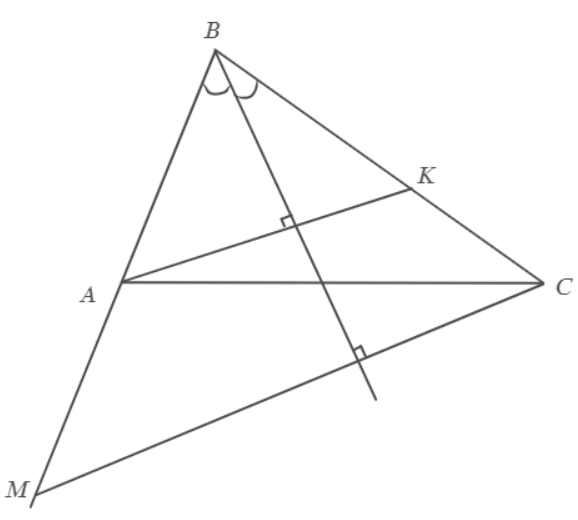
\includegraphics[scale=0.35]{g102.png}}
\end{figure}\\
В треугольниках $ABK$ и $MBC$ совпадают высота и биссектриса, поэтому они являются равнобедренными и $AB=BK,\ BM=BC.$ Возможны два случая расположения точек. В первом случае $AB=BK=BC-KC=BM-KC=8-1=7.$
 \begin{figure}[ht!]
\center{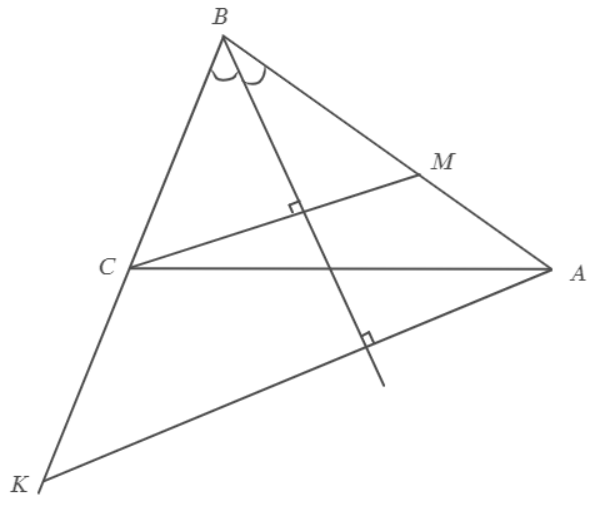
\includegraphics[scale=0.35]{g102-1.png}}
\end{figure}\\
Во втором случае $AB=BK=BC+KC=BM+KC=8+1=9.$
ewpage

oindent103.\begin{figure}[ht!]
\center{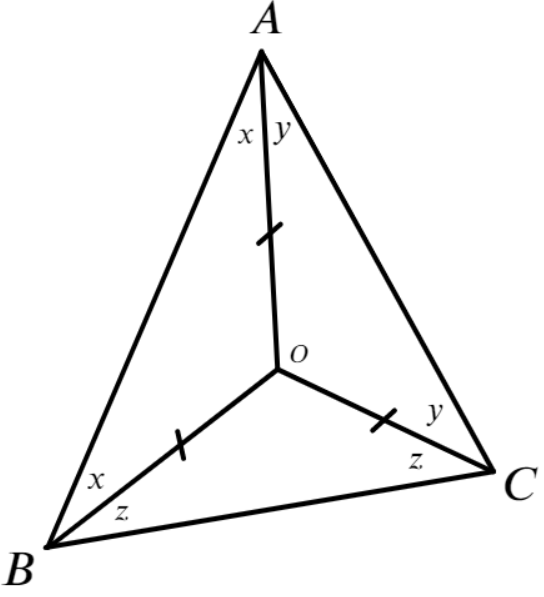
\includegraphics[scale=0.35]{g103.png}}
\end{figure}\\
Обозначим углы при основаниях этих равнобедренных треугольников буквами $x,\ y$ и $z.$ Тогда можно составить систему уравнений: $\begin{cases}x+y=30^\circ,\\
x+z=70^\circ,\\ y+z=80^\circ.\end{cases}$ Сложив все уравнения, получим $2x+2y+2z=30^\circ+70^\circ+80^\circ,\ x+y+z=90^\circ.$ Тогда $x=90^\circ-80^\circ=10^\circ,\ y=90^\circ-70^\circ=20^\circ,\ z=90^\circ-30^\circ=60^\circ.$ Таким образом, углы треугольника $AOB$ равны $10^\circ,\ 10^\circ, 180^\circ-2\cdot10^\circ=160^\circ,$ треугольника $AOC:\ 20^\circ,\ 20^\circ, 180^\circ-2\cdot20^\circ=140^\circ,$ треугольника $BOC:\ 60^\circ,\ 60^\circ, 180^\circ-2\cdot60^\circ=60^\circ.$\\
